\chapter{تبدیل متن به گفتار: مسئله و معماری خط‌لولهٔ \eng{TTS}}

\section{از تحلیل گفتار تا تولید گفتار}

\subsection{مرور جلسات گذشته}
تا این جلسه، محور درس \textbf{تحلیل سیگنال گفتار} بود: یک موج صوتی (\eng{waveform}) از پیش در اختیار ما بود و می‌کوشیدیم نمایش‌ها و ویژگی‌های گوناگونی از آن استخراج کنیم. موضوعاتی که تاکنون دیده‌ایم عبارت‌اند از:
\begin{itemize}
  \item \term{طیف‌نگار}{Spectrogram}: نمایش محتوای فرکانسی سیگنال در طول زمان؛
  \item \eng{MFCC}: ویژگی‌های صوتی فشرده بر پایهٔ مقیاس مل؛
  \item \term{پروزودی}{Prosody} و دو نمونهٔ آن، \term{کانتور گام}{Pitch Contour} و \term{کانتور شدت}{Intensity Contour}؛
  \item \term{فرمنت‌ها}{Formants} و نقش آن‌ها در تمایز آواها؛
  \item محل و شیوهٔ تولید آوا (\eng{Place/Manner of Articulation}) و پدیدهٔ \term{هم‌تولیدی}{Coarticulation}.
\end{itemize}
در همهٔ این مباحث «سیگنال» ورودی بود و «اطلاعات» خروجی. از این جلسه به بعد وارد سامانه‌های اصلی پردازش گفتار و زبان می‌شویم: تبدیل متن به گفتار (\eng{Text-to-Speech} یا \eng{TTS})، سامانه‌های گفت‌وگو (\eng{Dialogue Systems}) و تبدیل گفتار به متن (\eng{Speech-to-Text} یا \eng{STT}). موضوع این جلسه \term{تبدیل متن به گفتار}{Speech Synthesis} است.

\subsection{صورت مسئله}
در \eng{TTS} جهت مسئله معکوس می‌شود:
\[
\text{\lr{Text}} \;\longrightarrow\; \text{\lr{Speech Waveform}}
\]
یک متن داریم و باید از روی آن موجی بسازیم که شنونده آن را گفتار طبیعی و قابل فهم بداند. دو مشکل بنیادی در این مسیر وجود دارد.

\subsubsection{شکاف حجم اطلاعات}
متن در مقایسه با موج صوتی بسیار کم‌حجم است. اگر موج با نرخ نمونه‌برداری $f_s = 24\,000$ هرتز تولید شود، هر ثانیه گفتار ۲۴ هزار نمونه دارد؛ در مقابل، جملهٔ متناظر فقط چند ده نویسه یا واج است. پس پرسش اصلی این است: چگونه از یک نمایش بسیار کوتاه، توالی‌ای با ده‌ها هزار مقدار عددی بسازیم؟

\subsubsection{کم‌گویی متن}
متن همهٔ اطلاعات لازم برای گفتار طبیعی را در خود ندارد. برای نمونه معلوم نیست:
\begin{itemize}
  \item گوینده با چه لحنی صحبت کند؛
  \item کدام بخش جمله تأکید بگیرد؛
  \item سرعت بیان چقدر باشد و کجا مکث رخ دهد؛
  \item صدا متعلق به چه نوع گوینده‌ای باشد (جنسیت، سن، لهجه، ویژگی‌های صدای او).
\end{itemize}
بنابراین مدل تولید گفتار ناچار است بخشی از این اطلاعات را از دادهٔ آموزشی و بافت متن \textbf{استنتاج یا تولید} کند. به بیان دیگر، نگاشت متن به گفتار یک‌به‌یک نیست؛ یک متن را می‌توان به شیوه‌های بی‌شماری خواند (نگاشت یک‌به‌چند).

\begin{addedbox}{مثال عددی: شکاف نرخ‌ها برای یک جملهٔ سه‌ثانیه‌ای}
جمله‌ای معمولی را در نظر بگیرید که حدود \textbf{۳ ثانیه} طول می‌کشد و ۴۰ واج و حدود ۴۵ نویسه دارد. مقدارهای زیر را می‌توان با رابطهٔ $N = f_s \times T$ (تعداد نمونه = نرخ نمونه‌برداری × مدت) و با نرخ قاب‌بندی طیف‌نگار حساب کرد. فرض می‌کنیم طیف‌نگار مل ۸۰ بعدی با گام (\eng{hop}) ۳۰۰ نمونه در ۲۴ کیلوهرتز ساخته شده باشد (که با گام $12.5$ میلی‌ثانیه برابر است).
\begin{center}
\begin{tabular}{lcc}
\toprule
نمایش & تعداد مقدار در ۳ ثانیه & نرخ بر ثانیه \\
\midrule
نویسه‌ها & $\approx 45$ & $\approx 15$ \\
واج‌ها & $40$ & $\approx 13.3$ \\
قاب‌های طیف‌نگار مل & $72000/300 = 240$ & $80$ \\
مقدارهای طیف‌نگار مل & $240 \times 80 = 19\,200$ & $6400$ \\
نمونه‌های موج ($24$ کیلوهرتز) & $24000 \times 3 = 72\,000$ & $24\,000$ \\
\bottomrule
\end{tabular}
\end{center}
هر واج به‌طور میانگین $3\,\text{s}/40 = 75$ میلی‌ثانیه طول دارد؛ یعنی حدود ۶ قاب طیف‌نگار و حدود $72000/40 = 1800$ نمونهٔ موج. همچنین موج خام ۱۶ بیتی تک‌کاناله در ۲۴ کیلوهرتز حدود $24000 \times 16 = 384$ کیلوبیت بر ثانیه است؛ ۳ ثانیه یعنی حدود $1.15$ مگابیت. در سوی دیگر، اگر هر یک از ۴۰ واج را با دست‌بالا $\log_2 40 \approx 5.3$ بیت کدگذاری کنیم، به حدود ۲۱۳ بیت می‌رسیم. نسبت این دو ($\approx 5400$ برابر) نشان می‌دهد مدل باید چه حجم عظیمی از «جزئیات» را بسازد.
\end{addedbox}

\begin{figure}[htbp]
\centering
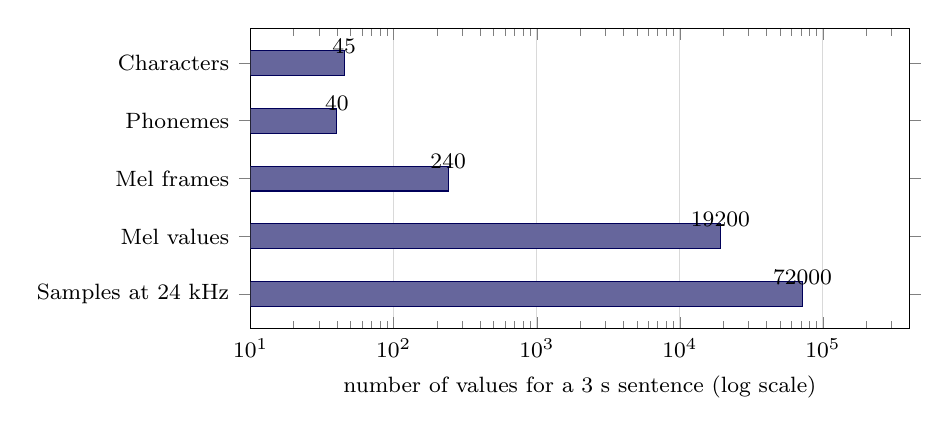
\begin{tikzpicture}
\begin{axis}[
  xbar, xmode=log, width=0.82\textwidth, height=5.4cm,
  xmin=10, xmax=400000,
  symbolic y coords={Samples at 24 kHz, Mel values, Mel frames, Phonemes, Characters},
  ytick=data, y tick label style={font=\footnotesize},
  x tick label style={font=\footnotesize},
  xlabel={\lr{number of values for a 3 s sentence (log scale)}},
  xlabel style={font=\footnotesize},
  nodes near coords, point meta=explicit symbolic, nodes near coords style={font=\footnotesize},
  bar width=9pt, enlarge y limits=0.15,
  xmajorgrids, grid style={gray!30},
]
\addplot[fill=blue!35!black!60, draw=blue!35!black] coordinates {
  (72000,Samples at 24 kHz) [72000] (19200,Mel values) [19200] (240,Mel frames) [240] (40,Phonemes) [40] (45,Characters) [45]
};
\end{axis}
\end{tikzpicture}
\caption{تعداد مقدارهای لازم برای نمایش یک جملهٔ سه‌ثانیه‌ای در سطح‌های مختلف؛ محور افقی لگاریتمی است و بین متن و موج چند مرتبهٔ بزرگی فاصله است. (شکل افزوده)}
\end{figure}

\section{دو رویکرد کلی: خط‌لوله و سرتاسری}

برای ساخت یک سامانهٔ \eng{TTS} دو رویکرد کلی وجود دارد.

\paragraph{رویکرد خط‌لوله‌ای (\eng{Pipeline-Based}).}
مسئله به چند بخش کوچک‌تر تقسیم می‌شود. هر ماژول وظیفهٔ مشخصی دارد و خروجی‌اش ورودی ماژول بعدی است. مزیت این ساختار آن است که هر بخش را می‌توان جداگانه بررسی، آموزش، اصلاح یا جایگزین کرد.

\paragraph{رویکرد سرتاسری (\eng{End-to-End}).}
هدف این است که یک مدل (یا مجموعه‌ای یکپارچه از لایه‌ها) متن را مستقیماً به گفتار تبدیل کند. در این حالت لزوماً همهٔ مراحل میانی به‌صورت ماژول‌های مستقل و قابل مشاهده وجود ندارند.

\begin{exambox}{نکتهٔ تأکیدی استاد}
رویکرد \eng{End-to-End} \textbf{لزوماً بهترین گزینه برای همهٔ کاربردها نیست}. گاهی به‌دلیل محدودیت‌هایی مانند تأخیر پردازش (\eng{Latency}) یا ویژگی‌های دامنهٔ کاربرد، استفاده از ماژول‌های کلاسیک یا یک خط‌لوله مناسب‌تر است. برای مثال ممکن است در یک کاربرد مشخص مرحلهٔ نرمال‌سازی متن بسیار حساس باشد و بخواهیم آن را مستقل از مدل تولید صوت بسازیم و تنظیم کنیم. در این جلسه تمرکز بر رویکرد خط‌لوله است؛ جزئیات معماری مدل‌ها و یک جلسهٔ جداگانه برای رویکردهای سرتاسری به جلسات بعد موکول شده است.
\end{exambox}

\begin{correctionbox}{«سرتاسری» یک طیف است}
واژهٔ \eng{End-to-End} در ادبیات \eng{TTS} همیشه یک معنا ندارد. برخی مدل‌ها فقط بخش «واج/نویسه به طیف‌نگار» را سرتاسری یاد می‌گیرند و برای ساخت موج هنوز به یک وکودر جدا نیاز دارند (مثلاً \eng{Tacotron 2}). مدل‌هایی هم مانند \eng{VITS} متن (یا واج) را در یک مدل یکپارچه به موج می‌رسانند. حتی در این حالت معمولاً یک بخش پیش‌پردازش متن (نرمال‌سازی و \eng{G2P}) بیرون از مدل باقی می‌ماند. پس انتخاب «خط‌لوله یا سرتاسری» دوگانهٔ مطلق نیست و بیشتر پرسش این است که مرز ماژول‌ها کجا کشیده شود.
\end{correctionbox}

\begin{addedbox}{نگاهی گذرا به تاریخچه و مثال‌ها}
سامانه‌های کلاسیک \eng{TTS} (ترکیب پیوندی \eng{concatenative/unit selection} و ترکیب آماری مبتنی بر \eng{HMM}) نیز خط‌لوله‌ای بودند. در دورهٔ شبکه‌های عصبی، \eng{Tacotron 2} (۲۰۱۷–۲۰۱۸) متن نویسه‌ای را با یک مدل دنباله‌به‌دنباله و توجه (\eng{attention}) به طیف‌نگار مل تبدیل می‌کرد و یک وکودر \eng{WaveNet} آن را به موج می‌رساند. \eng{FastSpeech} (۲۰۱۹) مدل آکوستیکی غیرخودهمبسته و سریع‌تری ارائه داد. \eng{HiFi-GAN} (۲۰۲۰) یک وکودر مبتنی بر \eng{GAN} سریع و باکیفیت است و \eng{VITS} (۲۰۲۱) یک مدل سرتاسری است که از متن/واج مستقیماً موج می‌سازد. جزئیات این مدل‌ها در جلسات بعد می‌آید.
\end{addedbox}

\section{معماری کلی یک سامانهٔ \eng{TTS}}

سامانهٔ \eng{TTS} را می‌توان به دو بخش اصلی تقسیم کرد.

\begin{description}
  \item[بخش اول: \eng{Front-End} یا تحلیل متن (\eng{Text Analysis}).] ورودی هنوز متن است و هدف، آماده‌سازی آن برای تولید گفتار است: به عبارتی تعیین اینکه «چه باید گفته شود» (\eng{what to say}). خروجی این بخش یک نمایش میانی، یعنی توالی واج‌ها (و در صورت نیاز اطلاعات پروزودی)، است.
  \item[بخش دوم: \eng{Back-End} یا تولید گفتار (\eng{Speech/Waveform Synthesis}).] نمایش واجی به نمایش آکوستیکی و سپس به موج تبدیل می‌شود: تعیین اینکه «چگونه گفته شود» (\eng{saying it}).
\end{description}

مسیر کلی پردازش چنین است:
\begin{center}
\begin{latin}
\small Text $\to$ Text Normalization $\to$ Homograph Disambiguation $\to$ G2P $\to$ Phonemes\\
$\to$ Acoustic Model $\to$ (Mel-)Spectrogram $\to$ Vocoder $\to$ Waveform
\end{latin}
\end{center}

\begin{figure}[htbp]
\centering
\resizebox{\textwidth}{!}{%
\begin{tikzpicture}[rtl, 
  box/.style={draw, rounded corners=3pt, minimum width=2.55cm, minimum height=1.0cm, align=center, fill=softblue, font=\small},
  data/.style={draw, rounded corners=1pt, minimum width=2.2cm, minimum height=0.8cm, align=center, fill=softyellow, font=\small},
  arr/.style={-{Stealth[length=2.5mm]}, thick},
  small/.style={font=\scriptsize, text=black!65, align=center}
]
% Front-end (right to left)
\node[data] (txt) at (12.2,0) {\rl{متن خام}\\\scriptsize\lr{Text}};
\node[box] (norm) at (9.1,0) {\rl{نرمال‌سازی متن}\\\scriptsize\lr{Text Normalization}};
\node[box] (homo) at (6.0,0) {\rl{رفع ابهام هم‌نویسه}\\\scriptsize\lr{Homograph Disamb.}};
\node[box] (g2p) at (2.9,0) {\rl{تبدیل نویسه به واج}\\\scriptsize\lr{G2P}};
\node[data] (ph) at (0,0) {\rl{توالی واج‌ها}\\\scriptsize\lr{Phonemes}};
\draw[arr] (txt) -- (norm);
\draw[arr] (norm) -- (homo);
\draw[arr] (homo) -- (g2p);
\draw[arr] (g2p) -- (ph);
% Back-end (left to right)
\node[box, fill=softgreen] (am) at (3.1,-2.7) {\rl{مدل آکوستیکی}\\\scriptsize\lr{Acoustic Model}};
\node[data] (mel) at (6.1,-2.7) {\rl{طیف‌نگار مل}\\\scriptsize\lr{Mel-Spectrogram}};
\node[box, fill=softgreen] (voc) at (9.1,-2.7) {\rl{وکودر}\\\scriptsize\lr{Vocoder}};
\node[data] (wav) at (12.2,-2.7) {\rl{موج گفتار}\\\scriptsize\lr{Waveform}};
\draw[arr] (ph.south) |- (am.west);
\draw[arr] (am) -- (mel);
\draw[arr] (mel) -- (voc);
\draw[arr] (voc) -- (wav);
% region labels
\draw[dashed, gray] (-1.4,0.95) rectangle (13.5,-0.95);
\node[anchor=south west, font=\small\bfseries, text=mainblue] at (-1.3,0.95) {\lr{Front-End: Text Analysis}};
\draw[dashed, gray] (1.7,-1.75) rectangle (13.5,-4.15);
\node[anchor=north west, font=\small\bfseries, text=mainblue] at (1.8,-4.2) {\lr{Back-End: Speech Generation}};
% size notes
\node[small] at (-0.9,-1.3) {\rl{$30$--$50$ واج}};
\node[small, anchor=north] at (6.1,-3.3) {\rl{$\approx 80$ قاب بر ثانیه}};
\node[small, anchor=north] at (12.2,-3.3) {\rl{$\approx 24000$ نمونه بر ثانیه}};
\end{tikzpicture}}
\caption{نمودار بلوکی خط‌لولهٔ \eng{TTS}: بخش تحلیل متن (بالا، جهت جریان از راست به چپ) و بخش تولید گفتار (پایین، از چپ به راست). مستطیل‌های زرد نمایش‌های دادهٔ میانی و مستطیل‌های رنگی ماژول‌های پردازشی‌اند. (شکل افزوده)}
\end{figure}

\boardfigure{0.95}{ch07-pipeline-board.png}{خط‌لولهٔ استاندارد \eng{TTS} در قالب ماژول‌های پردازشی و نمایش‌های میانی: متن، متن نرمال‌شده، متن آوانگاری‌شده، طیف‌نگار و موج گفتار.}

\subsection{خلاصهٔ نقش ماژول‌ها}
\begin{enumerate}
  \item \term{نرمال‌سازی متن}{Text Normalization}: تبدیل متن خام به متنی که بتوان آن را درست خواند (گسترش عدد، تاریخ، ساعت، واحد پول و اختصار به صورت کلمه).
  \item \term{رفع ابهام هم‌نویسه}{Homograph Disambiguation}: تعیین تلفظ درست کلماتی که نوشتار یکسان و تلفظ متفاوت دارند، با توجه به متن اطراف.
  \item \term{تبدیل نویسه به واج}{Grapheme-to-Phoneme, G2P}: تبدیل نمایش نوشتاری به نمایش واجی.
  \item \term{مدل آکوستیکی}{Acoustic Model}: تبدیل توالی واج‌ها به یک نمایش آکوستیکی مانند طیف‌نگار مل.
  \item \term{وکودر}{Vocoder}: تبدیل نمایش آکوستیکی به موج صوتی.
\end{enumerate}
مراحل ۱ تا ۳ بخش \eng{Front-End} و مراحل ۴ و ۵ بخش \eng{Back-End} را می‌سازند. بسته به معماری انتخاب‌شده ممکن است ترتیب، تفکیک یا ادغام برخی از این اجزا تفاوت کند.

\section{مرحلهٔ اول: نرمال‌سازی متن}

\subsection{چرا متن خام مستقیماً خواندنی نیست؟}
متن واقعی پر از عدد، تاریخ، ساعت، واحد پول، علامت اختصاری و عبارت‌هایی است که شکل نوشتاری‌شان با شکل گفتاری‌شان فرق دارد. در کلاس جملهٔ نمونه‌ای روی تخته نوشته شد که تقریباً همهٔ این پدیده‌ها را در خود داشت.

\begin{figure}[htbp]
\centering
\newcommand{\chmk}[2]{\tikz[baseline=(n.base)]{\node[draw=red!70!black,ellipse,inner xsep=1.5pt,inner ysep=0pt,line width=0.6pt](n){#2};\node[font=\tiny\bfseries,text=red!70!black,anchor=south west,inner sep=0.5pt] at (n.north east){\lr{#1}};}}
\fbox{\begin{minipage}{0.9\textwidth}
\medskip
\large\linespread{1.5}\selectfont
در تاریخ \chmk{1}{$1402/10/15$} ساعت \chmk{2}{$16{:}30$}، آن \chmk{3}{مرد} پس از مدت‌ها بیماری در بیمارستان \chmk{4}{مرد} و \chmk{5}{سرم} را از دستش کشیدند. \chmk{6}{خواهرم} گفت «\chmk{7}{سرم} به شدت درد می‌کند». حدود \chmk{8}{$2/5$} \chmk{9}{تن} گندم به ارزش \chmk{10}{۱۲۵} میلیون و \chmk{11}{۵۰۰} هزار \chmk{12}{تومان} با \chmk{13}{۳۰٪} تخفیف فروخته شد.
\medskip
\end{minipage}}

\medskip
\small
\begin{tabular}{@{}clll@{}}
\toprule
\textbf{شمارهٔ نشانه} & \textbf{نوع} & \textbf{شکل نوشتاری} & \textbf{شکل گفتاری (یادداشت استاد)}\\
\midrule
۱ & تاریخ & $1402/10/15$ & پانزدهم دی‌ماه هزار و چهارصد و دو\\
۲ & ساعت & $16{:}30$ & چهار و نیم (بعدازظهر) یا شانزده و سی دقیقه\\
۳ & هم‌نویسه (اسم) & مرد & \lr{mard} (انسان مذکر)\\
۴ & هم‌نویسه (فعل) & مرد & \lr{mord} (فوت کرد)\\
۵ & هم‌نویسه & سرم & \lr{sorom} (محلول تزریقی)\\
۶ & واژهٔ دارای ضمیر پیوسته & خواهرم & خواهر $+$ ـم (یادداشت حاشیه ناخوانا)\\
۷ & هم‌نویسه & سرم & \lr{saram} (سرِ من)\\
۸ & عدد اعشاری & $2/5$ & دو و نیم\\
۹ & واحد اندازه‌گیری & تن & تن\\
۱۰--۱۱ & عدد & ۱۲۵ و ۵۰۰ & صد و بیست و پنج میلیون و پانصد هزار\\
۱۲ & واحد پول & تومان & تومان (در گفتار محاوره‌ای: تومن)\\
۱۳ & درصد & ۳۰٪ & سی درصد\\
\bottomrule
\end{tabular}
\caption{جملهٔ نمونهٔ روی تخته و نشانه‌گذاری‌های استاد: تاریخ، ساعت، عددها، واحد پول، درصد، و دو هم‌نویسهٔ «مرد» و «سرم» که در جمله دو بار با تلفظ‌های متفاوت آمده‌اند. (بازسازی‌شده از تختهٔ کلاس)}
\end{figure}

برای خواندن این جمله، سامانه باید بداند که $1402/10/15$ یک تاریخ شمسی است و باید به‌شکل «پانزدهم دی‌ماه هزار و چهارصد و دو» خوانده شود؛ $16{:}30$ ساعت است و به‌شکل «شانزده و سی دقیقه» یا «چهار و نیم بعدازظهر» بیان می‌شود (هر دو یک زمان‌اند اما سبک بیانشان فرق دارد و سامانه باید آن را متناسب با کاربرد و سبک گفتار انتخاب کند)؛ $2/5$ در کنار «تن» یک عدد اعشاری است و «دو و نیم» خوانده می‌شود؛ ۳۰٪ یعنی «سی درصد». همچنین اگر سامانه برای گفتار محاوره‌ای ساخته شده باشد ممکن است «تومان» را «تومن» بخواند؛ این هم به سبک گفتار مطلوب بستگی دارد.

\begin{definitionbox}{هدف نرمال‌سازی در \eng{TTS}}
متن ورودی باید به شکلی تبدیل شود که سامانه بتواند آن را \textbf{درست و طبیعی بخواند}. به‌عبارتی، نرمال‌سازی در \eng{TTS} یعنی ساختن «شکل گفتاری» (\eng{spoken form}) از «شکل نوشتاری» (\eng{written form}).
\end{definitionbox}

\subsection{نرمال‌سازی در \eng{TTS} با نرمال‌سازی در \eng{NLP} فرق دارد}
استاد تأکید کرد که مفهوم نرمال‌سازی وابسته به هدف است. همیشه باید پرسید: «متن را نسبت به چه هدفی نرمال می‌کنیم؟»

در پردازش متن برای وظایف معمول \eng{NLP}، نرمال‌ساز (مثلاً در کتابخانهٔ \eng{Hazm}) معمولاً \term{کاهنده}{Reductive} است؛ یعنی تنوع نوشتاری را کم می‌کند تا متن برای فهم معنا یکدست شود. کارهای معمول آن:
\begin{itemize}
  \item تبدیل «ي» عربی به «ی» فارسی و «ك» عربی به «ک» فارسی؛
  \item اصلاح فاصله و نیم‌فاصله، مثلاً چسباندن پیشوندهای فعلی (تبدیل «می روم» به «می‌روم»)؛
  \item حذف تکرارهای غیرعادی حروف (مثلاً «سلاااام» به «سلام»)؛
  \item آماده‌سازی برای نشانه‌گذاری (\eng{tokenization}) و دیگر پردازش‌ها.
\end{itemize}
این کارها در کاربردهای زیر اهمیت دارند:
\begin{enumerate}
  \item \textbf{موتور جست‌وجو و بازیابی اطلاعات}: اگر کاربر «کتاب» را جست‌وجو کند، باید همهٔ شکل‌های نوشتاری آن (با «ک» عربی یا فارسی) یافت شود.
  \item \textbf{دسته‌بندی متن و تحلیل احساسات}: کاهش اندازهٔ واژگان تا مدل برای «می روم»، «میروم» و «می‌روم» سه بردار جدا نسازد.
  \item \textbf{استخراج موجودیت‌های نامدار (\eng{NER}) و برچسب‌گذاری اجزای کلام (\eng{POS Tagging})}: پیشوندها و پسوندها باید به بن واژه متصل باشند (مثلاً «می» جدا از «روم» نباشد).
\end{enumerate}

اما در \eng{TTS} هدف دیگری داریم: متن باید \textbf{خواندنی} شود. بسیاری از اطلاعاتی که نرمال‌سازِ \eng{NLP} دور می‌ریزد باید حفظ شوند و حتی اطلاعات تازه‌ای باید به متن اضافه شود تا خواندنش ممکن گردد. برای نمونه حذف \term{واژه‌های ایست}{Stopword} که در بعضی مراحل \eng{NLP} مفید است، برای \eng{TTS} نامناسب است، چون باید همهٔ محتوای جمله خوانده شود. به همین دلیل روی تخته دو نوع نرمال‌ساز مقابل هم قرار گرفتند: «کاهنده» در برابر «گسترش‌دهنده و آواشناسی‌محور» (\eng{Expansive \& Phonetic}).

\begin{warningbox}{دو نرمال‌ساز با یک نام}
نرمال‌ساز \eng{Hazm} و نرمال‌ساز لازم برای گفتار هدف‌های متفاوتی دارند: اولی \textbf{کاهنده} است و تنوع نوشتار را برای فهم معنا کم می‌کند؛ دومی \textbf{گسترش‌دهنده} است و متن را برای خواندن آماده می‌کند (عدد را به کلمه تبدیل می‌کند و اطلاعات تلفظی را روشن می‌کند). این دو را با هم اشتباه نگیرید.
\end{warningbox}

\begin{correctionbox}{تضاد مطلق نیست}
دوگانهٔ «کاهنده/گسترش‌دهنده» تصویری مفید اما کمی ساده‌شده است. یک سامانهٔ \eng{TTS} هم به یکدست‌سازی املایی نیاز دارد: وقتی تلفظ کلمات را در فرهنگ تلفظ جست‌وجو می‌کنیم، «ي/ی»، «ك/ک» و نیم‌فاصله‌های نادرست جست‌وجو را به‌هم می‌ریزند. تفاوت اصلی این است که \eng{TTS} علاوه بر آن به «گسترش» نیاز دارد و حق ندارد اطلاعاتی را که روی خواندن اثر می‌گذارند حذف کند؛ مثلاً علائم نگارشی (ویرگول و علامت سؤال) نشانه‌هایی برای مکث و آهنگ‌اند و نباید مثل بعضی پیش‌پردازش‌های \eng{NLP} حذف شوند.
\end{correctionbox}

\subsection{کلمات غیراستاندارد (\eng{NSW})}
هستهٔ نرمال‌سازی در \eng{TTS}، برخورد با \term{کلمات غیراستاندارد}{Non-Standard Words, NSW} است؛ توکن‌هایی که با نوشتارشان نمی‌توان تلفظشان را از روی قواعد معمول حدس زد. دسته‌های اصلی آن‌ها عبارت‌اند از: اعداد، تاریخ، ساعت، واحد پول، درصد، اختصارات، شماره‌ها و شناسه‌ها، و شکل‌های غیررسمی و عامیانهٔ نوشتار. روی تخته جمله‌ای نوشته شده بود که اصل کار را خلاصه می‌کند: «باید بفهمیم جزو چه دسته‌ای است؛ مثلاً عدد، واحد پول، تاریخ.»

\boardfigure{0.42}{ch07-norm-categories.png}{جدولی از ۲۷ دستهٔ نرمال‌سازی که روی تخته به‌عنوان نمونه نشان داده شد؛ مانند \eng{Cardinal}، \eng{Date}، \eng{Time}، \eng{Currency}، \eng{Telephone}، \eng{Abbreviations} و \eng{URL/Email}.}

\subsection{خواندن عدد بر اساس نوع آن}
یک توالی از ارقام را نمی‌توان با یک قاعدهٔ ثابت به کلمه تبدیل کرد؛ ابتدا باید \textbf{نوع و نقش} آن مشخص شود. در انگلیسی، مثلاً ۱۹۷۶ اگر سال باشد دو بخش «نوزده» و «هفتاد و شش» خوانده می‌شود، اما در یک شناسه ممکن است رقم‌به‌رقم یا به‌شکل دیگری خوانده شود. در فارسی هم این مسئله هست:

\begin{center}
\small
\begin{tabular}{llp{6.6cm}}
\toprule
نوع & نمونه & شکل گفتاری \\
\midrule
عدد اصلی & ۱۲۵ & صد و بیست و پنج \\
سال & ۱۴۰۲ & هزار و چهارصد و دو \\
تاریخ & $1402/10/15$ & پانزدهم دی‌ماه هزار و چهارصد و دو \\
ساعت & $16{:}30$ & شانزده و سی دقیقه، یا چهار و نیم بعدازظهر \\
عدد اعشاری & $2/5$ (در کنار «تن») & دو و نیم \\
مبلغ & ۱۲۵ میلیون و ۵۰۰ هزار تومان & صد و بیست و پنج میلیون و پانصد هزار تومان \\
درصد & ۳۰٪ & سی درصد \\
شناسه یا شماره تلفن & رشتهٔ ارقام & رقم‌به‌رقم یا گروه‌گروه، مثلاً «صفر نه یک دو …» \\
\bottomrule
\end{tabular}
\end{center}

\begin{warningbox}{یک نویسه، چند نقش}
علامت «/» در جملهٔ نمونه سه نقش دارد: در $1402/10/15$ جداکنندهٔ اجزای تاریخ است، در $2/5$ ممیز اعشاری است (در همین قالب ممکن بود یک تاریخ یا یک کسر باشد) و در متن‌های دیگر ممکن است «یا» باشد. تنها نشانهٔ تفکیک، بافت است: واژهٔ «تن» پس از $2/5$ قرینهٔ خوانش اعشاری است. ابهام مشابهی در سال (۱۴۰۲ به‌صورت «هزار و چهارصد و دو» و نه «چهارده و صفر دو») و در خوانش‌های دیگر دیده می‌شود.
\end{warningbox}

\subsection{روش کلاسیک پیاده‌سازی}
برای پیاده‌سازی این مرحله، یک الگوی کلاسیک دو بخشی پیشنهاد شد:
\begin{enumerate}
  \item \textbf{طبقه‌بندی توکن} (\eng{Token Classification}): مشخص می‌کنیم هر توکن به کدام دسته تعلق دارد (عدد، تاریخ، ساعت، پول و ...).
  \item \textbf{مبدل} (\eng{Converter}): پس از تعیین دسته، مبدل مخصوص آن دسته توکن را به شکل گفتاری تبدیل می‌کند.
\end{enumerate}
\[
\text{\lr{Input Token}} \to \text{\lr{Token Classification}} \to \text{\lr{Category-Specific Converter}} \to \text{\lr{Spoken Form}}
\]

برای طبقه‌بندی می‌توان از عبارت‌های باقاعده (\eng{Regular Expression})، قواعد دستی، کتابخانه‌های آماده یا مدل‌های یادگیری ماشین استفاده کرد. در کلاس به کتابخانهٔ \eng{num2fawords} اشاره شد که عدد را به حروف فارسی درمی‌آورد؛ برای نمونه خروجی تابع words(170) برابر است با «یکصد و هفتاد». استاد تأکید کرد که این کتابخانه فقط برای دستهٔ \textbf{اعداد} است و برای تاریخ، ساعت یا اختصارها باید مبدل جدا داشت. اگر برای یک دسته کتابخانه یا قاعدهٔ آماده وجود نداشته باشد، می‌توان دادهٔ آموزشی تهیه کرد، یک طبقه‌بند ساخت و خروجی آن را به مبدل همان دسته داد.

\boardfigure{0.5}{ch07-num2fawords.png}{نمونهٔ استفاده از کتابخانهٔ \eng{num2fawords}: تبدیل عدد ۱۷۰ به حروف.}

\begin{addedbox}{مثال عددی: مبدل اعداد کمتر از هزار}
قاعدهٔ مبدل برای عدد $n<1000$ را می‌توان با سه جدول نوشت: صدگان (صد، دویست، سیصد، چهارصد، پانصد، ششصد، هفتصد، هشتصد، نهصد)، دهگان (بیست، سی، ... ، نود، و دهه‌های ده تا نوزده به‌صورت واژه‌های جدا) و یکان. سپس اجزای ناصفر با «و» به هم وصل می‌شوند.
\begin{itemize}
  \item $125 \leftarrow$ صدگان: «صد»، دهگان: «بیست»، یکان: «پنج» $\Leftarrow$ «صد و بیست و پنج».
  \item $500 \leftarrow$ «پانصد».
  \item $1402 \leftarrow$ «هزار» + $402$ $\Leftarrow$ «هزار و چهارصد و دو» (و نه «چهارده صد و دو»؛ خوانش دورقمی‌دورقمی مخصوص سال در انگلیسی است).
  \item $125\,500\,000 \leftarrow$ «صد و بیست و پنج میلیون و پانصد هزار».
\end{itemize}
آنچه در متن «۱۲۵ میلیون و ۵۰۰ هزار تومان» آمده در واقع مجموع دو گروه است: $125 \times 10^6 + 500 \times 10^3 = 125\,500\,000$. مبدل باید «میلیون» و «هزار» را به‌عنوان واحدهای مقیاس بشناسد و ضرایبشان را جداگانه تبدیل کند.
\end{addedbox}

\begin{addedbox}{پیاده‌سازی مبتنی بر \eng{WFST}}
در سامانه‌های صنعتی، قاعده‌های نرمال‌سازی اغلب با \term{مبدل‌های متناهی وزن‌دار}{Weighted Finite-State Transducer, WFST} نوشته می‌شوند. هر دستهٔ توکن یک دستور زبان (گرامر) مبدل دارد؛ مثلاً یک مبدل رقم را به واژه تبدیل می‌کند و مبدل دیگری قالب تاریخ را می‌شناسد. این مبدل‌ها را می‌توان ترکیب (\eng{composition}) کرد و وزن‌ها (هزینه‌ها) برای انتخاب میان چند خوانش ممکن (مثلاً «شانزده و سی» در برابر «چهار و نیم») به کار می‌روند. سامانه‌هایی مانند \eng{Kestrel/Sparrowhawk} از این رویکرد استفاده می‌کنند. مزیت: قاعده‌ها قابل‌بازرسی و کنترل‌اند و تأخیر کم است؛ عیب: نوشتن و نگهداری قاعده‌ها برای زبان و دامنهٔ جدید پرزحمت است و پوشش بافت‌های پیچیده محدود می‌ماند.
\end{addedbox}

\subsection{اهمیت دامنهٔ کاربرد}
فراوانی کلمات غیراستاندارد در متن‌های مختلف یکسان نیست. در کلاس سه نوع داده با هم مقایسه شد: متن خبری رسمی (\eng{New York Times})، متن شبکه‌های اجتماعی (\eng{Twitter}) و پیام‌های کوتاه (\eng{SMS}). نمودار روی تخته، توزیع نسبت توکن‌های خارج از واژگان (\eng{OOV}) در هر پیام را نشان می‌دهد.

\boardfigure{0.8}{ch07-oov-corpora.png}{احتمال دیدن پیامی با نسبت معین از توکن‌های \eng{OOV} در سه پیکره. در متن خبری بیشتر پیام‌ها (حدود ۴۸ درصد) هیچ توکن \eng{OOV} ندارند؛ در توییتر حدود ۳۱ درصد و در \eng{SMS} فقط حدود ۱۵ درصد. زیرنویس تصویر: «در توییتر ۱۵ درصد توییت‌ها ۵۰ درصد یا بیشتر \eng{OOV} دارند.» (مقدارهای تقریبی خوانده‌شده از نمودار)}

نتیجه‌ای که روی تخته نوشته شد: هرچه به ارتباطات غیررسمی (توییتر و \eng{SMS}) نزدیک‌تر شویم، \eng{NSW}ها (اختصارها، املای غیررسمی و اصطلاحات عامیانه) شایع‌تر می‌شوند. هیچ‌یک از این پیکره‌ها ۱۰۰ درصد غیراستاندارد نیست؛ در متن خبری احتمال نبودن \eng{OOV} بسیار بالاست، در حالی که در توییتر با احتمال خوبی نیمی از توکن‌ها غیراستانداردند.

اهمیت این مشاهده برای طراحی سامانه: اگر شکل صحیح خواندن یک عبارت تشخیص داده نشود، گفتار تولیدشده غیرطبیعی یا حتی غلط می‌شود (مثلاً خواندن یک تاریخ مثل چند عدد جدا). این یکی از مزیت‌های خط‌لوله است: \textbf{اهمیت و پیچیدگی هر ماژول به دامنه وابسته است}. اگر سامانه برای پیام‌های کوتاه یا شبکه‌های اجتماعی طراحی می‌شود باید روی نرمال‌سازی بیشتر سرمایه‌گذاری کرد؛ اگر ورودی عمدتاً متن رسمی و استاندارد است، این مرحله را می‌توان ساده‌تر گرفت.

\begin{correctionbox}{\eng{OOV} و \eng{NSW} یکی نیستند}
نمودار شمارش توکن‌های «خارج از واژگان» (\eng{OOV}) را نشان می‌دهد، در حالی که \eng{NSW} توکنی است که تلفظش از نوشتارش مستقیماً به دست نمی‌آید. این دو هم‌پوشانی زیادی دارند (عددها، اختصارها، املای عامیانه معمولاً در فرهنگ واژگان نیستند) اما یکسان نیستند: مثلاً اشتباه تایپی هم \eng{OOV} است ولی لزوماً \eng{NSW} نیست. در کلاس \eng{OOV} به‌عنوان شاخصی برای فراوانی \eng{NSW} به کار رفت و برای نتیجهٔ کلی همین کافی است.
\end{correctionbox}

\section{مرحلهٔ دوم: رفع ابهام هم‌نویسه‌ها}

پس از نرمال‌سازی، مسئلهٔ مهم دیگری باقی است: برخی کلمات نوشتار یکسان اما تلفظ متفاوت دارند. این کلمات \term{هم‌نویسه}{Homograph} نام دارند. (\eng{Grapheme} به نویسه، یعنی واحد نوشتاری، اشاره دارد؛ پس هم‌نویسه یعنی «نویسه‌های یکسان».)

\begin{definitionbox}{هم‌نویسه (\eng{Homograph})}
دو یا چند واژه که املای (نویسهٔ) یکسان دارند ولی تلفظ‌شان فرق می‌کند، و معمولاً معنی‌شان نیز فرق دارد. در \eng{TTS} هدف از \term{رفع ابهام هم‌نویسه}{Homograph Disambiguation} انتخاب تلفظ درست با توجه به بافت جمله است.
\end{definitionbox}

\subsection{نمونه‌های فارسی}
ریشهٔ بسیاری از هم‌نویسه‌های فارسی این است که مصوت‌های کوتاه (\eng{a}، \eng{e}، \eng{o}) در نوشتار معمولی نشان داده نمی‌شوند.

\begin{center}
\begin{tabular}{lll}
\toprule
نوشتار & تلفظ‌های ممکن (\eng{IPA}) & معنی \\
\midrule
مرد & \eng{[mæɾd]} / \eng{[moɾd]} & انسان مذکر (اسم) / فوت کرد (فعل) \\
کرم & \eng{[keɾm]} / \eng{[keɾem]} & کرم خاکی / کرم مرطوب‌کننده؛ همچنین \eng{[kæɾæm]} (بخشش) \\
سرم & \eng{[seɾom]} / \eng{[sæɾæm]} & محلول پزشکی / «سرِ من» \\
\bottomrule
\end{tabular}
\end{center}
در جملهٔ نمونهٔ روی تخته، «مرد» در یک جمله دو بار با دو تلفظ آمده بود («آن \underline{مَرد} ... در بیمارستان \underline{مُرد}») و «سرم» نیز دو بار: «\underline{سِرُم} را از دستش کشیدند» و «\underline{سَرَم} به شدت درد می‌کند». خواننده با نقش دستوری و معنی جمله به‌سادگی تلفظ را درمی‌یابد؛ سامانه باید همین توانایی را به دست آورد.

\subsection{دو راه برای رفع ابهام}
\paragraph{راه اول: اطلاعات نحوی (\eng{Syntactic Information}).}
گاهی نقش دستوری واژه تلفظ درست را مشخص می‌کند. ابزار این کار \term{برچسب‌گذاری اجزای کلام}{Part-of-Speech Tagging} یا \eng{POS Tagging} است که برای هر کلمه نقش اسم، فعل، صفت، قید، ضمیر و ... را تعیین می‌کند. در تخته نمونه‌ای با \eng{Hazm} دیده شد: برای جملهٔ «ما بسیار کتاب می‌خوانیم» برچسب‌ها به‌ترتیب ضمیر (\eng{PRO})، قید (\eng{ADV})، اسم (\eng{N}) و فعل (\eng{V}) است.

\boardfigure{0.7}{ch07-hazm-pos.png}{برچسب‌گذاری اجزای کلام با \eng{Hazm}: ما (ضمیر)، بسیار (قید)، کتاب (اسم)، می‌خوانیم (فعل).}

بنابراین در جملهٔ «آن مَرد رفت» برچسب‌گذار «مرد» را اسم می‌شناسد و در «او مُرد» فعل. این تفاوت نحوی تلفظ را روشن می‌کند.

\paragraph{راه دوم: بافت و معنا (\eng{Context}).}
اگر دو واژه نقش دستوری یکسان داشته باشند (مثلاً «کِرم» خاکی و «کِرِم» مرطوب‌کننده هر دو اسم‌اند)، برچسب‌گذاری کمکی نمی‌کند و باید معنای جمله، یعنی کلمات پیش و پس و مفهوم کلی، به کار گرفته شود. یک راه یادگیری ماشینی، استفاده از \term{نمایش بافتی}{Contextual Embedding} است: بردار هر کلمه با توجه به جملهٔ اطراف ساخته می‌شود، پس یک کلمه در دو جملهٔ متفاوت می‌تواند دو بردار متفاوت داشته باشد. (جزئیات این نمایش‌ها در جلسات بعد می‌آید.)

\subsection{مدلی برای رفع ابهام هم‌نویسه}
روی تخته یک مدل نمونه برای رفع ابهام هم‌نویسه نشان داده شد. جملهٔ ورودی («او با نفس گرم خودش روح داد») کلمه به کلمه از یک مدل \eng{Embedding} می‌گذرد؛ نمایش کلمهٔ هدف («گرم»، با بردار \eng{E4}) به یک طبقه‌بند داده می‌شود و طبقه‌بند فقط میان تلفظ‌های \textbf{مرتبط با همان کلمه} (در شکل: \eng{garm} و \eng{geram}) بیشینه می‌گیرد.

\boardfigure{0.62}{ch07-homograph-model.png}{مدل نمونهٔ رفع ابهام هم‌نویسه: مدل \eng{Embedding} بردار بافتی هر واژه را می‌سازد و طبقه‌بند، تنها میان تلفظ‌های نامزد کلمهٔ هدف («گَرم» یا «گِرِم») بیشینه می‌گیرد.}

\paragraph{یک طبقه‌بند مشترک در برابر طبقه‌بند جدا برای هر کلمه.}
روی تخته توضیح داده شده بود که چرا یک طبقه‌بند سراسری (\eng{Global Classifier}) برای همهٔ هم‌نویسه‌ها بهتر از یک طبقه‌بند جدا برای هر کلمه است. خلاصه:
\begin{itemize}
  \item هم‌نویسه‌ها در قواعد نحوی، ساختاری و معنایی زبان مشترک‌اند؛ مثلاً: «اگر قبل از کلمه حرف تعریف، ضمیر ملکی یا صفت آمد، یا کلمه در جایگاه فاعل/مفعول نشست، این کلمه اسم است؛ پس نامزدی را فعال کن که برچسب اسمی دارد.»
  \item اگر برای هر کلمه یک طبقه‌بند جدا بود، روی کلمات کم‌تکرار بیش‌برازش (\eng{Overfit}) رخ می‌داد یا اصلاً چیزی یاد نمی‌گرفت.
  \item با وزن‌های مشترک (\eng{Shared Weights})، مدل توانایی تشخیص فاعل، مفعول، حرف اضافه و ساختار زبان را از کلمات پرتکرار یاد می‌گیرد و همان دانش را مستقیماً روی کلمات کم‌تکرار به کار می‌برد؛ این همان \term{یادگیری انتقالی میان‌کلمه‌ای}{Cross-word Transfer Learning} است.
\end{itemize}

\begin{addedbox}{«بیشینه گرفتن فقط روی تلفظ‌های مرتبط» یعنی چه؟}
فرض کنید طبقه‌بند سراسری $N$ کلاس (تلفظ) دارد و برای کلمهٔ هدف $w$ تنها زیرمجموعهٔ $C(w)$ از آن‌ها مجاز است. احتمال هر کلاس بر پایهٔ نمرهٔ خام (\eng{logit}) $z_c$ چنین ساخته می‌شود:
\[
p(c \mid w, \text{بافت}) = \frac{e^{z_c}}{\sum_{c' \in C(w)} e^{z_{c'}}}, \qquad c \in C(w),
\]
و تلفظ نهایی $\hat c = \arg\max_{c \in C(w)} p(c \mid \cdot)$ است. مثلاً اگر $C(\text{گرم}) = \{\text{garm},\text{geram}\}$ و $z_{\text{garm}} = 2$ و $z_{\text{geram}} = 0$، آنگاه $p(\text{garm}) = e^{2}/(e^{2}+e^{0}) \approx 0.88$ و تلفظ انتخابی «garm» است. کلاس‌های نامربوط (مثلاً تلفظ‌های کلمات دیگر) هرگز انتخاب نمی‌شوند.
\end{addedbox}

\begin{exambox}{پرسش روی تخته: «اینجا \eng{Argmax} یا تصادفی؟»}
در نمودار مدل، استاد پرسید خروجی نهایی با \eng{argmax} انتخاب شود یا به‌صورت تصادفی. در رفع ابهام هم‌نویسه هدف یافتن تلفظ \textbf{درست و قطعی} است، پس انتخاب معمول \eng{argmax} روی نامزدهای مجاز است؛ نمونه‌برداری تصادفی بیشتر برای تنوع در خروجی‌های تولیدی (مثلاً پروزودی) مطرح می‌شود.
\end{exambox}

\subsection{ارتباط با \eng{WSD}}
این مسئله به \term{رفع ابهام معنایی واژه}{Word Sense Disambiguation, WSD} نزدیک است. در \eng{WSD} می‌خواهیم معنای درست واژه در جمله را تعیین کنیم؛ مثلاً «شیر» می‌تواند جانور، نوشیدنی یا شیر آب باشد. رفع ابهام هم‌نویسه نیز از بافت و معنا استفاده می‌کند، اما هدفش مشخص‌تر است: تعیین \textbf{تلفظ} درست.

\begin{correctionbox}{هر ابهام معنایی ابهام تلفظی نیست}
هر سه معنای «شیر» در فارسی \eng{[ʃiɾ]} تلفظ می‌شوند. پس «شیر» یک ابهام معنایی (\eng{WSD}) است ولی برای \eng{TTS} هم‌نویسه محسوب نمی‌شود: تلفظ یکسان است و ابهام معنایی تأثیری در تولید گفتار ندارد (واژه‌هایی که املا و تلفظ یکسان و معنی متفاوت دارند «هم‌آوا-هم‌نویسه» یا \eng{homonym} هستند). بنابراین رفع ابهام هم‌نویسه فقط به آن بخشی از \eng{WSD} نیاز دارد که به تفاوت تلفظ می‌انجامد. اطلاعات معنایی ابزاری است برای رسیدن به تلفظ صحیح.
\end{correctionbox}

\section{تبدیل نویسه به واج (\eng{G2P})}

پس از نرمال‌سازی و رفع ابهام، باید متن را به نمایشی تبدیل کنیم که برای تولید صوت مناسب باشد. تا اینجا ورودی ما توالی نویسه‌ها (\eng{Grapheme}) بود؛ برای تولید گفتار به \term{واج}{Phoneme} نیاز داریم. این تبدیل را \term{نویسه‌به‌واج}{Grapheme-to-Phoneme, G2P} می‌نامند: نگاشت نویسه‌های نرمال‌شده به واج‌ها.

\subsection{نویسه و واج}
\begin{definitionbox}{نویسه و واج}
\textbf{نویسه (\eng{Grapheme})}: واحد تمایزدهندهٔ نظام نوشتاری یک زبان، مانند حروف الفبا («س»، «ل»، \eng{a}، \eng{b}). \\
\textbf{واج (\eng{Phoneme})}: کوچک‌ترین واحد صوتی تمایزدهنده در نظام آوایی زبان؛ صداهایی که با الفبای آوانگاری مانند \eng{IPA} یا \eng{ARPAbet} نوشته می‌شوند.
\end{definitionbox}

\begin{correctionbox}{نویسه «معنادار» نیست}
روی تخته نویسه «کوچک‌ترین واحد معنادار خط» توصیف شده بود. دقیق‌تر آن است که بگوییم نویسه کوچک‌ترین واحد \textbf{متمایزکنندهٔ} نظام نوشتاری است؛ «معنادار بودن» ویژگی \term{تکواژ}{Morpheme} است، نه نویسه. حرف «س» به‌تنهایی معنایی ندارد؛ فقط با حرف‌های دیگر واژه‌ای را از واژهٔ دیگر جدا می‌کند.
\end{correctionbox}

\subsection{آیا نگاشت نویسه به واج یک‌به‌یک است؟}
نه. در بعضی زبان‌ها رابطهٔ نوشتار و تلفظ منظم‌تر است و در بعضی استثنا بیشتر. انگلیسی هم نگاشت یک‌به‌یک ندارد (مثلاً \eng{tion} که «\eng{ʃən}» خوانده می‌شود). در فارسی هم نیاز به \eng{G2P} روشن است:
\begin{itemize}
  \item مصوت‌های کوتاه در نوشتار معمولی نمایش داده نمی‌شوند، اما هنگام تلفظ وجود دارند و باید در نمایش واجی بیایند؛ استاد روی تخته «کتاب» را به‌صورت \eng{ketab} و «شب» را به‌صورت \eng{ʃab} نوشت.
  \item پدیده‌هایی مانند تشدید (که واج را تکرار می‌کند) و سکون و نیز استثنا‌های املایی که نوشتار با تلفظ تطابق ندارد باید در نظر گرفته شوند.
  \item بعضی نویسه‌ها چند تلفظ دارند (مثلاً «و» می‌تواند /v/، /u/، /o/ یا /ow/ باشد) و بعضی واج‌ها چند نویسه (/s/ با «س»، «ص»، «ث»؛ /z/ با «ز»، «ذ»، «ض»، «ظ»).
\end{itemize}

\subsection{پیش‌نیازهای طراحی یک سامانهٔ \eng{G2P}}
روی تخته سه پرسش اساسی طرح شده بود:
\begin{enumerate}
  \item \textbf{با چه نمادهایی تلفظ را نشان دهیم؟} انتخاب \term{الفبای آوانگاری}{Phonetic Alphabet}؛ مثلاً \eng{IPA}.
  \item \textbf{برای هر واژه چه تلفظی ثبت شده است؟} انتخاب \term{فرهنگ تلفظ}{Pronunciation Dictionary}؛ منبعی که نوشتار را به تلفظ نگاشت می‌کند و هم برای یادگیری و هم برای سنجش خروجی مدل به کار می‌رود.
  \item \textbf{چگونه از روی نوشتار تلفظ را پیش‌بینی کنیم؟} انتخاب \textbf{مدل \eng{G2P}}؛ مثلاً مدل‌های دنباله‌به‌دنبالهٔ رمزگذار–رمزگشا (\eng{Encoder–Decoder}) که توالی نویسه‌ها را می‌گیرند و توالی واج‌ها را تولید می‌کنند. معماری این مدل‌ها بعداً بررسی می‌شود.
\end{enumerate}

\subsection{الفبای آوایی بین‌المللی (\eng{IPA})}
\eng{IPA} (\eng{International Phonetic Alphabet}) بر این اصل بنا شده که برای هر صدای متمایز گفتاری یک نماد جدا وجود داشته باشد («یک صدا، یک نماد»؛ \eng{One sound, one symbol}). جدول \eng{IPA} نمادها را بر پایهٔ همان ویژگی‌های تولیدی‌ای که در جلسات پیشین دیدیم سازمان می‌دهد: ردیف‌های جدول شیوهٔ تولید (انسدادی، خیشومی، سایشی، ...) و ستون‌هایش محل تولید (دولبی، دندانی، لثوی، نرم‌کامی، ...) است. بخش مصوت‌ها نیز بر پایهٔ ارتفاع و پیشین/پسین‌بودن زبان چیده شده، که همان فضای مصوت و فرمنت‌های \eng{F1} و \eng{F2} است. البته همهٔ خانه‌های جدول در فارسی وجود ندارد. همچنین هم‌تولیدی باعث می‌شود تولید واقعی یک آوا از آواهای مجاورش اثر بپذیرد، پس نمایش واجی توصیف دقیق همهٔ جزئیات آوایی نیست.

\coursefigure{0.72}{ch07-ipa-chart.png}{جدول الفبای آوایی بین‌المللی (\eng{IPA}، بازبینی‌شده در ۲۰۰۵) که در کلاس نمایش داده شد.}

\begin{table}[htbp]
\centering
\begin{tabular}{lll}
\toprule
\textbf{نوشتار} & \textbf{نمایش واجی (\eng{IPA})} & \textbf{نکته}\\
\midrule
کتاب & \lr{ketab} & مصوت‌های کوتاه در نوشتار نیامده‌اند\\
شب & \lr{ʃab} & «ش» با نماد \lr{ʃ} نمایش داده می‌شود\\
\bottomrule
\end{tabular}
\caption{دو نمونهٔ نگاشت نوشتار به واج که استاد در حاشیهٔ جدول \eng{IPA} نوشت. (بازسازی‌شده از تختهٔ کلاس)}
\end{table}

\subsection{ابزارها و منابع}
\begin{itemize}
  \item \eng{phonemizer}: بستهٔ پایتونی که متن را به واج‌های \eng{IPA} تبدیل می‌کند (برای نمونه خروجی عبارت \eng{hello world} برابر است با \eng{həloʊ wɜːld}).
  \item \eng{KaamelDict}: فرهنگ تلفظ فارسی (\eng{Persian G2P Dictionary}) روی \eng{Hugging Face} که هر ورودی آن یک نویسه‌رشته و توالی واجی‌اش است.
  \item \eng{Persian Phonetic Corpus}: پیکره‌ای که متن فارسی را در سطح واژه و سطح جمله با \eng{IPA} آوانگاری کرده است.
\end{itemize}

\boardfigure{0.55}{ch07-phonemizer.png}{ابزار \eng{phonemizer}: تبدیل متن انگلیسی به واج‌های \eng{IPA} با یک فرمان.}

\boardfigure{0.8}{ch07-kaameldict.png}{نمونه‌ای از فرهنگ \eng{KaamelDict}: هر سطر یک واژهٔ فارسی (نویسه) و فهرست واج‌های متناظرش را دارد؛ این فرهنگ نمادهای \eng{ASCII}ـمحور برای واج‌ها به کار می‌برد (برای مثال \eng{S} به‌جای \eng{ʃ} و \eng{A} برای مصوت بلند \eng{/ɑː/}، بر پایهٔ ورودی‌های نمایش‌داده‌شده).}
\label{fig:ch07-kaameldict}

\boardfigure{0.9}{ch07-persian-phonetic-sent.png}{پیکرهٔ آوانگاری‌شدهٔ فارسی در سطح جمله؛ تلفظ پیوستهٔ یک جملهٔ کامل با \eng{IPA}.}

\subsection{طرح عملی پیشنهادی: چه موقع از کدام روش استفاده کنیم؟}
روی تخته یک نمودار تصمیم برای کل بخش نویسه‌به‌واج رسم شده بود. کلمهٔ ورودی ابتدا از جهت \eng{OOV} بودن بررسی می‌شود:
\begin{itemize}
  \item \textbf{اگر در فرهنگ تلفظ نباشد (\eng{OOV})}: از یک مدل رمزگذار–رمزگشا که در سطح بایت کار می‌کند (\eng{ByT5}) استفاده می‌شود. این مدل بر روی تلفظ کلمات فرهنگ آموزش می‌بیند و نوشتار را در سطح بایت‌های \eng{UTF-8}، یعنی کاراکتر به کاراکتر، می‌خواند؛ پس از قید «یک کلمه» آزاد می‌شود. وابستگی‌اش به واژه شکسته می‌شود و توان تعمیم به کلمات دیده‌نشده پیدا می‌کند: انتظار داریم قواعد پنهان آوایی زبان را یاد بگیرد (مثلاً در انگلیسی \eng{tion} را «\eng{ʃ}» بخواند، حتی اگر بخشی از واژه \eng{OOV} باشد).
  \item \textbf{اگر در فرهنگ باشد}: بررسی می‌شود که هم‌نویسه است یا نه؛ اگر هست، طبقه‌بند سراسری رفع ابهام تلفظ درست را برمی‌گزیند. اگر نیست، تلفظ ثبت‌شده در فرهنگ (یا قواعد دستی/کتابخانه‌های آماده) به کار می‌رود.
\end{itemize}

\begin{figure}[htbp]
\centering
\resizebox{\textwidth}{!}{%
\begin{tikzpicture}[rtl, 
  dec/.style={draw=mainblue, thick, diamond, aspect=2.4, fill=softyellow, align=center, inner sep=2pt, font=\normalsize},
  box/.style={draw=mainblue, thick, rounded corners=3pt, fill=softblue, align=center, minimum height=1.1cm, minimum width=3.2cm, font=\normalsize},
  arr/.style={-{Stealth[length=2.8mm]}, thick, mainblue},
  lab/.style={font=\small, fill=white, inner sep=1.5pt},
  note/.style={draw=black!45, dashed, rounded corners=2pt, align=center, font=\footnotesize, text=black!75, inner sep=3pt}
]
\node[dec] (oov) at (4.6,0) {\lr{OOV?}};
\node[dec] (hom) at (9.4,-2.6) {هم‌نویسه؟};
\node[box, fill=softgreen, minimum width=4.2cm] (byt5) at (0.4,-2.6) {\lr{ByT5}\\\lr{Encoder--Decoder}};
\node[box] (glob) at (7.0,-5.2) {\lr{Global Classifier}};
\node[box] (lib) at (11.6,-5.2) {کتابخانه‌ها /\\دست‌ساز};
\draw[arr] (oov.west) -- node[lab, above left] {بله} (byt5.north);
\draw[arr] (oov.east) -- node[lab, above right] {خیر} (hom.north);
\draw[arr] (hom.south west) -- node[lab, above left] {بله} (glob.north);
\draw[arr] (hom.south east) -- node[lab, above right] {خیر} (lib.north);
\node[note] (n1) at (0.4,-4.7) {\rl{آموزش روی تلفظ واژه‌های فرهنگ}\\\rl{خواندن در سطح بایت‌های \lr{UTF-8}}\\\rl{حالت نهایی رمزگذار (\lr{Context Vector}) به رمزگشا می‌رود}};
\draw[dashed, black!45] (byt5.south) -- (n1.north);
\node[note] (q1) at (-0.6,-0.1) {\rl{پرسش روی تخته:}\\\rl{«تسک چیست؟»}};
\draw[dashed, black!45] (q1.south) -- (byt5.north west);
\node[note] (q2) at (7.0,-6.9) {\rl{پرسش روی تخته:}\\\rl{«اینجا \lr{Argmax} یا نمونه‌گیری تصادفی؟»}};
\draw[dashed, black!45] (glob.south) -- (q2.north);
\end{tikzpicture}}
\caption{نمودار تصمیم برای بخش تلفظ: کلمهٔ \eng{OOV} به مدل \eng{ByT5} (رمزگذار–رمزگشا) می‌رود؛ کلمهٔ هم‌نویسه به طبقه‌بند سراسری؛ در غیر این صورت از کتابخانه/فرهنگ دست‌ساز استفاده می‌شود. دو پرسش مطرح‌شده روی تخته نیز با کادر خط‌چین نشان داده شده است. (بازسازی‌شده از تختهٔ کلاس)}
\end{figure}

\begin{addedbox}{چرا مدل در سطح بایت؟}
هر حرف فارسی در \eng{UTF-8} معمولاً ۲ بایت است و هر حرف لاتین ۱ بایت. مدلی که بایت‌ها را می‌خواند واژگان بسیار کوچکی (کمتر از ۳۰۰ نماد) دارد و هرگز با «کلمهٔ ناشناخته» روبه‌رو نمی‌شود؛ چون در این سطح همهٔ رشته‌ها قابل نمایش‌اند. این برخلاف مدل‌های سطح واژه است که برای هر واژهٔ نادیده فقط یک نشانهٔ «ناشناخته» دارند. مدل \eng{ByT5} (۲۰۲۱) نسخهٔ بایتی \eng{T5} است. به همین دلیل برای \eng{G2P} روی کلمات \eng{OOV} گزینهٔ مناسبی است.
\end{addedbox}

\begin{exambox}{پایان بخش تحلیل متن}
در پایان \eng{G2P} خروجی ما یک \textbf{توالی واجی} است. در این نقطه بخش \eng{Text Analysis} (\eng{Front-End}) پایان می‌یابد و وارد مرحلهٔ تولید صوت (\eng{Back-End}) می‌شویم.
\end{exambox}

\section{مرحلهٔ دوم سامانه: تولید گفتار از روی واج‌ها}

ورودی این بخش مجموعه‌ای از واج‌هاست و خروجی‌اش موج گفتار. سه چالش اصلی پیش رو است.

\subsection{چالش اول: اطلاعات پروزودی}
متن لحن و آهنگ گفتار را به‌طور کامل مشخص نمی‌کند. در جلسهٔ گذشته دیدیم که پروزودی لایهٔ مهمی از گفتار است. مثلاً جملهٔ «سلام» می‌تواند عادی، پرسشی، همراه با تعجب یا با تأکید و احساس خاص گفته شود؛ کلمات یکسان‌اند اما خروجی صوتی متفاوت است. بخشی از این اطلاعات را می‌توان از نشانه‌های نگارشی (مثلاً علامت سؤال) یا بافت جمله به دست آورد، اما همیشه کافی نیست. بنابراین مدل باید بخشی از پروزودی را استنتاج کند یا امکان دریافت آن را به‌صورت کنترل‌های جدا داشته باشد (نوع صدا، سبک، حالت بیان). هدف آن است که صدا طبیعی‌تر شود و حالت رباتی نداشته باشد.

\subsection{چالش دوم: اختلاف نرخ و ابعاد نمایش‌ها}
فرض کنید خروجی \eng{G2P} برای یک جمله ۳۰ واج باشد و بخواهیم یک موج سه‌ثانیه‌ای با نرخ نمونه‌برداری ۲۴ کیلوهرتز بسازیم. تعداد نمونه‌های خروجی:
\[
N = f_s \times T = 24000 \times 3 = 72\,000 .
\]
یعنی «۳۰ واج ورودی $\leftarrow$ $72\,000$ نمونهٔ صوتی خروجی» (روی تخته: جملهٔ معمولی ۳۰ تا ۵۰ فونیم دارد). این اختلاف نشان می‌دهد که تولید گفتار نیازمند افزایش شدید وضوح زمانی است. در کلاس به این مسئله «\eng{Upsampling}» گفته شد. اما مسئله فقط زیادکردن تعداد نمونه نیست؛ مدل باید مقدار هر نمونه را هم به‌گونه‌ای تعیین کند که گفتار طبیعی و قابل فهم شود.

\begin{correctionbox}{نرخ ۲۴ کیلوهرتز و واژهٔ «\eng{Upsampling}»}
(الف) نرخ نمونه‌برداری «استاندارد» واحدی برای گفتار وجود ندارد: تلفن ۸ کیلوهرتز، تشخیص گفتار معمولاً ۱۶ کیلوهرتز، و در پژوهش‌های \eng{TTS} رایج‌ترین نرخ‌ها $22.05$ و ۲۴ کیلوهرتز (و در محصولات تجاری تا $44.1$ یا ۴۸ کیلوهرتز) است. عدد ۲۴ کیلوهرتز مثال معقولی است؛ \eng{Tacotron 2} روی ۲۴ کیلوهرتز کار می‌کند و \eng{HiFi-GAN} و \eng{VITS} روی دادهٔ $22.05$ کیلوهرتزی. \\
(ب) «\eng{Upsampling}» در این معنا یک اصطلاح تقریبی است: در عمل افزایش طول در دو جا رخ می‌دهد؛ ابتدا گسترش \textbf{واج به قاب} (چند قاب برای هر واج، با مدل‌سازی مدت) و سپس افزایش \textbf{قاب به نمونه} (هر قاب مل به‌اندازهٔ گام، یعنی چند صد نمونه، گسترش می‌یابد؛ این بخش \eng{upsampling} به معنای دقیق پردازش سیگنال با لایه‌های کانولوشن تراگذار است).
\end{correctionbox}

\subsection{چالش سوم: تطابق زمانی (\eng{Temporal Alignment})}
فرض کنید ۳۰ واج داریم. باید مشخص کنیم:
\begin{itemize}
  \item هر واج چه زمانی شروع شود و چه مدت ادامه یابد؛
  \item مرز دو واج کجاست؛
  \item کدام واج‌ها بر یکدیگر اثر می‌گذارند (هم‌تولیدی).
\end{itemize}
این موضوع به \term{مدل‌سازی مدت}{Duration Modeling} و \term{هم‌ترازی زمانی}{Temporal Alignment} مربوط است. همهٔ واج‌ها مدت یکسان ندارند (برخی کوتاه‌تر و برخی کشیده‌ترند) و به‌دلیل هم‌تولیدی مرز آواها هرگز کاملاً مجزا و مستقل نیست. پس سامانهٔ تولید گفتار علاوه بر ترتیب واج‌ها باید زمان‌بندی مناسب آن‌ها را نیز یاد بگیرد.

\begin{figure}[htbp]
\centering
\resizebox{\textwidth}{!}{%
\begin{tikzpicture}[rtl, 
  data/.style={font=\large},
  gbox/.style={draw=black!70, rounded corners=6pt, fill=softgreen, align=center, inner sep=8pt, font=\normalsize},
  arr/.style={-{Stealth[length=2.6mm]}, thick, mainblue}
]
\node[data] (t) at (0,0) {\lr{Text / Phonemes}};
\node[data] (s) at (7.2,0) {\lr{Spectrogram (Mel)}};
\node[data] (w) at (13.6,0) {\lr{Raw Waveform}};
\draw[arr] (t.east) -- node[above, font=\small] {\lr{Acoustic Model}} (s.west);
\draw[arr] (s.east) -- node[above, font=\small] {\lr{Vocoder}} (w.west);
\node[gbox] (c1) at (6.3,-3.2) {\rl{\textbf{چالش عدم تطابق نرخ نمونه‌برداری:}}\\[2pt]
\rl{جملهٔ معمولی حاوی حدود ۳۰ تا ۵۰ فونیم است.}\\
\rl{سیگنال خام صوتی با کیفیت استاندارد (۲۴ هزار هرتز) برای جملهٔ}\\
\rl{حدود ۳ ثانیه $=$ $72\,000$ نقطه/نمونه (\lr{Sample}) دارد.}\\[6pt]
\rl{\textbf{راه‌حل:} استفاده از اسپکتروگرام به‌عنوان یک نمایش میانی}\\
\rl{(\lr{Intermediate Representation}) که برای تقلیل پیچیدگی مسئله به کار رفته بوده است.}};
\node[gbox] (c2) at (10.5,-7.0) {\rl{\textbf{چالش‌ها:}}\\[2pt]
\rl{(عدم تطابق زمانی)}\\ \lr{Coarticulation}\\ \lr{Prosodic information}};
\draw[arr] (s.south) -- (s.south |- c1.north);
\end{tikzpicture}}
\caption{چالش‌های بخش \eng{Back-End}: مسیر «واج $\leftarrow$ طیف‌نگار مل $\leftarrow$ موج»، چالش اختلاف نرخ نمونه‌برداری و راه‌حل «نمایش میانی»، و فهرست چالش‌ها: عدم تطابق زمانی، هم‌تولیدی و اطلاعات پروزودی. (بازسازی‌شده از تختهٔ کلاس)}
\end{figure}

\section{مدل آکوستیکی}

برای ساده‌کردن مسئله، تولید گفتار به دو مرحله تقسیم می‌شود:
\[
\text{\lr{Phonemes}} \xrightarrow{\;\text{\lr{Acoustic Model}}\;} \text{\lr{Mel-Spectrogram}} \xrightarrow{\;\text{\lr{Vocoder}}\;} \text{\lr{Waveform}}
\]
\term{مدل آکوستیکی}{Acoustic Model} از روی واج‌ها یک نمایش آکوستیکی (مانند طیف‌نگار مل) می‌سازد. در این مرحله باید زمان‌بندی، ویژگی‌های آکوستیکی و در صورت لزوم ویژگی‌های پروزودی در تولید نمایش خروجی لحاظ شود.

\subsection{چرا طیف‌نگار به‌عنوان نمایش میانی؟}
پرسش طبیعی: چرا مستقیماً از واج به موج نرویم؟ پاسخ مطرح‌شده در کلاس این است که یک نمایش میانی \textbf{پیچیدگی مسئلهٔ یادگیری را کاهش می‌دهد}. به‌جای آنکه مدل مجبور باشد همهٔ جزئیات موج را در یک گام بسازد، ابتدا نمایشی ساختاریافته‌تر از ویژگی‌های صوتی تولید می‌کند و سپس ماژول دیگری آن را به موج برمی‌گرداند.

\begin{exambox}{مثال استاد: مسیر تهران تا مشهد}
فرض کنید فقط می‌دانیم کسی از تهران به مشهد رفته و مسافت مشخصی را طی کرده است. می‌خواهیم مسیر دقیقش را بازسازی کنیم. از مبدأ، مقصد و مسافت می‌توان اطلاعاتی گرفت، اما هنوز جزئیات بسیاری معلوم نیست: از کدام شهرها گذشته؟ کدام جاده‌ها را رفته؟ در تولید گفتار هم دانستن توالی واج‌ها برای مشخص‌شدن همهٔ جزئیات موج کافی نیست. اگر در میانهٔ راه «نقاط عطف» داشته باشیم (مثل شهرهای بین راه)، بازسازی مسیر ساده‌تر می‌شود. طیف‌نگار نقش همین نقاط عطف را دارد: اطلاعات بیشتری برای مرحلهٔ بعد فراهم می‌کند و بازسازی موج را ساده‌تر می‌سازد.
\end{exambox}

\begin{addedbox}{چرا دقیقاً طیف‌نگار مل؟}
چند دلیل فنی این انتخاب را رایج کرده است:
\begin{itemize}
  \item \textbf{کاهش طول}: با نرخ $22.05$ کیلوهرتز و گام ۲۵۶ نمونه (\eng{hop length})، نرخ قاب‌ها $22050/256 \approx 86.1$ قاب بر ثانیه است، یعنی ۲۵۶ بار کمتر از نرخ نمونه. برای ۳ ثانیه: $\lfloor 3 \times 86.13 \rfloor = 258$ قاب در برابر $66\,150$ نمونه.
  \item \textbf{فشردگی بعد فرکانسی}: طیف‌نگار خطی با پنجرهٔ ۱۰۲۴ نقطه‌ای ۵۱۳ مقدار برای هر قاب دارد، اما مل با ۸۰ فیلتر تنها ۸۰ مقدار (مقیاس مل بر پایهٔ ادراک شنوایی؛ جلسهٔ پیشین).
  \item \textbf{هموار و قابل پیش‌بینی بودن}: طیف‌نگار مل، برخلاف موج، ساختاری دارد که مدل می‌تواند آن را یاد بگیرد (هارمونیک‌ها، فرمنت‌ها، مرز واج‌ها).
  \item \textbf{جداسازی وظایف}: وکودر را می‌توان جدا از متن و روی داده‌های گفتاری بدون متن آموزش داد؛ همان وکودر برای مدل‌های آکوستیکی مختلف قابل استفاده است.
\end{itemize}
\end{addedbox}

\subsection{نقش \eng{Embedding} در مدل آکوستیکی}
در کلاس مثال زده شد که برای هر واج می‌توان یک بردار \term{تعبیه}{Embedding} در نظر گرفت؛ مثلاً هر واج با یک بردار ۵۱۲ بعدی. این عدد فقط مثالی از ابعاد \eng{Embedding} است. در آموزش، مدل نمایش‌هایی می‌آموزد که اطلاعات مربوط به هر واج و ارتباطش با واج‌های قبل و بعد را در خود دارند. در نتیجه مدل فقط به هویت یک واج مستقل محدود نیست و می‌تواند با استفاده از بافت مجاور، بخشی از اطلاعات لازم برای تولید طبیعی آن را بیاموزد. این موضوع به‌ویژه در پدیدهٔ هم‌تولیدی اهمیت دارد.

\begin{addedbox}{تصویر ذهنی از جدول \eng{Embedding}}
\eng{Embedding} یک جدول جست‌وجو است: اگر واژگان $V$ واج داشته باشد و بعد تعبیه $d=512$ باشد، جدول $E \in \mathbb{R}^{V \times 512}$ است و واج شمارهٔ $i$ به بردار سطر $i$ام ($e_i\in\mathbb{R}^{512}$) نگاشته می‌شود. با $V \approx 40$ واج فارسی، فقط $40 \times 512 = 20\,480$ پارامتر داریم. این بردارها در آموزش و همراه با بقیهٔ شبکه یاد گرفته می‌شوند. برای نمونه، در \eng{Tacotron 2} نیز نویسه‌ها به بردار ۵۱۲ بعدی نگاشت می‌شوند. اثر بافت (مثلاً هم‌تولیدی) در لایه‌های بعدی شبکه، مانند \eng{LSTM} دوسویه یا بلوک‌های \eng{Transformer}، وارد می‌شود: خروجی این لایه‌ها برای واج $i$ تابعی از واج‌های همسایه نیز هست.
\end{addedbox}

\subsection{مدل آکوستیکی و پروزودی}
استاد تأکید کرد که «تولید طیف‌نگار» و «پیش‌بینی پروزودی» دقیقاً یک مسئله نیستند. برای یک محتوای زبانی ثابت می‌توان حالت‌های پروزودی گوناگونی در نظر گرفت. بنابراین در بعضی معماری‌ها از مؤلفه‌های جدا برای پیش‌بینی ویژگی‌های پروزودی و تولید نمایش آکوستیکی استفاده می‌شود. مثلاً می‌توان برای یادگیری پروزودی یک تابع هزینه (\eng{Loss}) و برای خروجی آکوستیکی تابع هزینهٔ دیگری تعریف کرد تا مدل هم «چه گفته شود» و هم «چگونه گفته شود» را یاد بگیرد. نحوهٔ دقیق این تفکیک به معماری بستگی دارد.

\begin{addedbox}{مثال معماری‌ها}
\eng{FastSpeech 2} نمونه‌ای از این تفکیک است: علاوه بر خروجی طیف‌نگار، پیش‌بین‌های جداگانه‌ای برای \textbf{مدت}، \textbf{گام} (\eng{pitch}) و \textbf{انرژی} دارد که هرکدام تابع هزینهٔ مخصوص خود را دارند. \eng{FastSpeech} با یک «تنظیم‌کنندهٔ طول» (\eng{length regulator}) هر واج را به تعداد قاب‌های پیش‌بینی‌شده تکرار می‌کند؛ این همان حل مسئلهٔ هم‌ترازی زمانی به شیوهٔ صریح است. در \eng{Tacotron 2}، به‌جای مدت‌های صریح، سازوکار توجه (\eng{attention}) ضمنی هم‌ترازی را یاد می‌گیرد و پروزودی را از داده می‌آموزد.
\end{addedbox}

\section{وکودر: از طیف‌نگار به موج}

پس از تولید طیف‌نگار هنوز موج واقعی نداریم. ماژولی که نمایش آکوستیکی را به \eng{Waveform} تبدیل می‌کند \term{وکودر}{Vocoder} نام دارد (از «\eng{Voice + coder}»):
\[
\text{\lr{Spectrogram}} \xrightarrow{\;\text{\lr{Vocoder}}\;} \text{\lr{Waveform}}.
\]
(واژهٔ \eng{vocoder} به دههٔ ۱۹۳۰ و کارهای آزمایشگاه‌های بل برمی‌گردد؛ در \eng{TTS} امروزی منظور وکودر عصبی است.)

\subsection{چرا ساختن موج از طیف‌نگار ساده نیست؟}
پاسخ به تبدیل فوریه‌ای برمی‌گردد که در جلسات پیش دیدیم. ضرایب تبدیل فوریه هم \textbf{دامنه} دارند و هم \textbf{فاز}. اگر یک ضریب را به‌صورت $X = a + jb$ بنویسیم، اندازه و فاز آن چنین‌اند:
\[
|X| = \sqrt{a^{2}+b^{2}}, \qquad \phi = \text{\lr{atan2}}(b,a).
\]
طیف‌نگار فقط اندازه (\eng{Magnitude}) را نگه می‌دارد و فاز را کنار می‌گذارد. پس اگر فقط $|X|$ را داشته باشیم، نمی‌توانیم بدون اطلاعات یا تخمین اضافی، همهٔ جزئیات موج اولیه را بازیابیم. فاز مشخص می‌کند هر مؤلفهٔ فرکانسی کجای زمان قرار دارد و چگونه با بقیهٔ مؤلفه‌ها ترکیب می‌شود. روی تخته این مطلب چنین نوشته شده بود: «زاویه و زمان‌بندی (فاز) دور ریخته شد؛ علامت‌ها و نوسان‌های ریز مثبت/منفی (دامنهٔ لحظه‌ای موج) همه به عددهای مثبتِ "شدت انرژی" تبدیل شدند.»

\begin{addedbox}{مثال عددی: اندازه یکسان، فاز متفاوت}
دو ضریب مختلط $X_1 = 3+4j$ و $X_2 = -3+4j$ را در نظر بگیرید.
\begin{align*}
|X_1| &= \sqrt{9+16} = 5, & \phi_1 &= \text{\lr{atan2}}(4,3) \approx 53.1^\circ,\\
|X_2| &= \sqrt{9+16} = 5, & \phi_2 &= \text{\lr{atan2}}(4,-3) \approx 126.9^\circ .
\end{align*}
اندازه‌ها برابرند و تنها فاز آن‌ها متفاوت است؛ پس از روی اندازهٔ ۵ نمی‌توانیم بگوییم ضریب اصلی $X_1$ بوده یا $X_2$. شکل زیر همین نکته را روی سیگنال نشان می‌دهد: دو سیگنال از سه مؤلفهٔ سینوسی با فرکانس‌های ۲۰۰، ۵۰۰ و ۱۱۰۰ هرتز ساخته شده‌اند که دامنه‌هایشان برابر است و فقط فازشان فرق دارد. طیف اندازهٔ دو سیگنال دقیقاً یکی است اما شکل موج‌ها کاملاً متفاوت است.
\end{addedbox}

\coursefigure{0.92}{ch07-phase-demo.png}{دو سیگنال با طیف اندازهٔ یکسان و فازهای متفاوت: ردیف بالا شکل موج و ردیف پایین طیف اندازه است. طیف اندازه به‌تنهایی شکل موج را مشخص نمی‌کند و باید فاز را بازسازی یا تخمین زد. (شکل افزوده)}

\subsection{مسئلهٔ بازسازی فاز}
چون در طیف‌نگار اندازه‌ای فاز وجود ندارد، برای ساختن موج باید راهی برای بازسازی یا تولید یک سیگنال سازگار با آن پیدا کرد. دو دسته راه‌حل را می‌توان نام برد:
\begin{itemize}
  \item \textbf{روش‌های کلاسیک مانند \eng{Griffin–Lim}}: به‌طور تکراری فاز را حدس می‌زنند تا طیف‌نگار حاصل از سیگنال با طیف‌نگار مفروض سازگار شود. بدون آموزش و ساده‌اند، اما خروجی معمولاً صدایی مصنوعی و «وزوزی» دارد.
  \item \textbf{وکودرهای عصبی}: شبکهٔ عصبی مستقیماً از طیف‌نگار به موج می‌رسد و فاز را ضمنی یاد می‌گیرد. نمونه‌ها: \eng{WaveNet} (خودهمبستهٔ نمونه‌به‌نمونه و کند)، \eng{HiFi-GAN} (سریع و مبتنی بر \eng{GAN}).
\end{itemize}

\begin{correctionbox}{فاز «کاملاً» از بین نمی‌رود، اما بازیابی‌اش آسان نیست}
جملهٔ «اندازه را که نگه دارید، فاز حذف می‌شود» درست است، ولی دو دقت لازم است. (الف) طیف‌نگار بر پایهٔ پنجره‌های هم‌پوشان ساخته می‌شود، پس افزونگی دارد و می‌توان از ثبات میان قاب‌های متوالی (سازگاری \eng{STFT}) فاز را تا حد خوبی تخمین زد؛ \eng{Griffin–Lim} دقیقاً این کار را می‌کند. (ب) طیف‌نگار مل علاوه بر حذف فاز، تفکیک فرکانسی را هم کم می‌کند (بیش از ۵۰۰ نقطه به ۸۰ فیلتر)، پس بازگرداندن به طیف خطی هم تقریبی است. نتیجه: ساخت موج از مل یک مسئلهٔ تقریباً بدوضع‌طرح‌شده است که با یک مدل مولد خوب حل می‌شود.
\end{correctionbox}

\subsection{مدل‌های مولد و \eng{GAN}}
یکی از رویکردهای تولید موج استفاده از \term{شبکهٔ مولد رقابتی}{Generative Adversarial Network, GAN} است. معماری \eng{GAN} دو بخش دارد:
\begin{itemize}
  \item \term{مولد}{Generator}: خروجی مصنوعی (اینجا موج) می‌سازد؛
  \item \term{تمایزدهنده}{Discriminator}: می‌کوشد خروجی ساخته‌شده را از نمونهٔ واقعی تشخیص دهد.
\end{itemize}
بازخورد تمایزدهنده به بهتر شدن مولد کمک می‌کند. در پاسخ به پرسشی در کلاس، استاد روشن کرد که لازم نیست مدل \eng{GAN} یک «فاز» مستقل به‌عنوان خروجی تولید کند؛ می‌تواند مستقیماً موج صوتی بسازد و با تابع‌های هزینه، کیفیت را بهتر کند. هدف نهایی وکودر تولید موجی است که از نظر صوتی با نمایش ورودی سازگار باشد. جزئیات معماری‌های مولد و توابع هزینه به جلسات بعد موکول شد.

\begin{addedbox}{نگاهی گذرا به \eng{WaveNet} و \eng{HiFi-GAN}}
\textbf{\eng{WaveNet}} (۲۰۱۶): مدلی خودهمبسته (\eng{autoregressive}) با کانولوشن‌های علّی و متسع‌شده (\eng{dilated causal convolution}) که هر نمونه را به‌شرط نمونه‌های پیشین (و شرط‌های ورودی مانند طیف‌نگار مل) پیش‌بینی می‌کند؛ کیفیت خیلی بالا ولی تولید نمونه‌به‌نمونه، بسیار کند است. \\
\textbf{\eng{HiFi-GAN}} (۲۰۲۰): مولد کانولوشنی که با لایه‌های کانولوشن تراگذار، طول طیف‌نگار را به طول موج می‌رساند (در پیکربندی رایج با گام ۲۵۶، یعنی ضریب افزایش طول ۲۵۶) و دو دسته تمایزدهنده (چندمقیاسی و چنددوره‌ای) برای ارزیابی اجزای مختلف شکل موج دارد. برخلاف \eng{WaveNet} همهٔ نمونه‌ها را موازی تولید می‌کند و بسیار سریع‌تر از زمان واقعی است. \\
مثال ابعاد: برای یک مل ۸۰ بعدی با ۲۵۸ قاب، مولد باید ماتریس $258 \times 80 = 20\,640$ مقداری را به بردار $258\times 256 = 66\,048$ نمونه تبدیل کند (حدود ۳ ثانیه در $22.05$ کیلوهرتز). \\
\textbf{\eng{VITS}} (۲۰۲۱) این دو مرحله را درون یک مدل سرتاسری ترکیب می‌کند و رمزگذار متن، مدل مدت، و یک رمزگشای مشابه \eng{HiFi-GAN} را با هم آموزش می‌دهد.
\end{addedbox}

\section{جمع‌بندی خط‌لولهٔ \eng{TTS}}

جدول زیر خلاصهٔ مسیر را نشان می‌دهد:
\begin{center}
\small
\begin{tabular}{llll}
\toprule
مرحله & ورودی & خروجی & وظیفه \\
\midrule
\eng{Text Normalization} & متن خام & متن قابل خواندن & گسترش \eng{NSW} \\
\eng{Homograph Disamb.} & متن دارای هم‌نویسه & تلفظ مشخص‌شده & رفع ابهام بافتی و نحوی \\
\eng{G2P} & نویسه‌ها & واج‌ها & تبدیل نوشتار به نمایش واجی \\
\eng{Acoustic Model} & توالی واج‌ها & طیف‌نگار (مل) & تولید نمایش آکوستیکی \\
\eng{Vocoder} & طیف‌نگار & موج & تولید موج گفتار \\
\bottomrule
\end{tabular}
\end{center}
دو بخش اصلی: \textbf{\eng{Front-End}} (آماده‌سازی و تحلیل متن تا رسیدن به واج‌ها) و \textbf{\eng{Back-End}} (تولید نمایش آکوستیکی و موج از واج‌ها).

\subsection{چرا خط‌لوله هنوز مهم است؟}
ممکن است گمان کنیم چون مدل‌های \eng{End-to-End} وجود دارند دیگر نیازی به بررسی خط‌لوله نیست. استاد توضیح داد که این نتیجه‌گیری درست نیست. در برخی کاربردها کنترل مستقل هر بخش اهمیت دارد. برای مثال ممکن است بخواهیم:
\begin{itemize}
  \item نرمال‌ساز متن را برای یک دامنهٔ خاص تنظیم کنیم؛
  \item برای کاهش تأخیر از روشی سریع‌تر استفاده کنیم؛
  \item بخشی از سامانه را با مدل کلاسیک پیاده کنیم؛
  \item روی یک مشکل مشخص مانند اعداد یا هم‌نویسه‌ها تمرکز بیشتری داشته باشیم.
\end{itemize}
در خط‌لوله هر بخش مستقل‌تر قابل اصلاح و جایگزینی است. در مقابل، مدل‌های سرتاسری یکپارچه‌ترند و مزیت‌های دیگری در یادگیری و تولید دارند. انتخاب معماری باید بر پایهٔ مسئله و محدودیت‌های کاربرد انجام شود.

\subsection{جلسات آینده و گفت‌وگوی پایانی}
هدف این جلسه آشنایی با کل معماری \eng{TTS} و نقش هر ماژول بود، نه ورود به جزئیات همهٔ مدل‌ها. در جلسات آینده معماری‌های مختلف هر بخش، چه روش‌های کلاسیک و چه مدل‌های یادگیری عمیق، بررسی می‌شوند و یک جلسه به رویکردهای \eng{End-to-End} اختصاص می‌یابد.

\begin{exambox}{پرسش و پاسخ پایانی و نکات ارزیابی}
در پایان کلاس استاد پرسید آیا بهتر است پیش از ورود به مدل‌های اصلی مفاهیمی مانند \eng{Transformer}، \eng{Self-Attention}، \eng{Cross-Attention}، \eng{Encoder–Decoder} و \eng{GAN} نیز جداگانه توضیح داده شوند یا هنگام معرفی هر معماری به‌اندازهٔ لازم گفته شوند. پس از گفت‌وگو با دانشجویان قرار شد این مفاهیم به‌اندازهٔ لازم توضیح داده شوند تا هنگام معرفی مدل‌های بعدی بتوان به آن‌ها ارجاع داد. استاد اشاره کرد که مطالب تدریس‌شده می‌توانند در ارزیابی و امتحان مطرح شوند. تکلیف یا تمرین مشخصی در این جلسه اعلام نشد.
\end{exambox}

\section{جمع‌بندی}
در این جلسه از تحلیل سیگنال به \textbf{تولید} سیگنال رسیدیم. مسئلهٔ \eng{TTS} از دو جهت دشوار است: متن بسیار کم‌حجم‌تر از موج است و در عین حال اطلاعات پروزودی و گوینده را نیز ندارد. برای مهار این پیچیدگی، سامانه را به دو بخش \eng{Front-End} (نرمال‌سازی، رفع ابهام هم‌نویسه، \eng{G2P}) و \eng{Back-End} (مدل آکوستیکی و وکودر) تقسیم کردیم. در بخش اول، «خواندنی کردن» متن مهم است و با نرمال‌سازی مرسوم در \eng{NLP} فرق دارد؛ فراوانی \eng{NSW}ها به دامنه وابسته است و تلفظ هم‌نویسه‌ها به نقش دستوری و بافت. در بخش دوم، طیف‌نگار مل به‌عنوان نمایش میانی، پیچیدگی تبدیل واج به موج را کم می‌کند و وکودر باید فازِ ازدست‌رفته را بازسازی کند. این جلسه چارچوبی ایجاد کرد که معماری‌های دقیق مدل‌ها در جلسات بعد در آن جای می‌گیرند.

\begin{exambox}{نکات مهم برای مرور و امتحان}
\begin{enumerate}
  \item در \eng{TTS} مسیر برعکس تحلیل گفتار است: متن $\leftarrow$ موج. چالش‌ها: شکاف حجم اطلاعات، کم‌گویی متن، و نگاشت یک‌به‌چند.
  \item دو رویکرد: \eng{Pipeline} و \eng{End-to-End}؛ سرتاسری بودن لزوماً بهتر نیست (تأخیر، دامنه، کنترل).
  \item دو بخش: \eng{Front-End} (متن $\leftarrow$ واج) و \eng{Back-End} (واج $\leftarrow$ طیف‌نگار $\leftarrow$ موج).
  \item نرمال‌سازی در \eng{TTS} گسترش‌دهنده و آواشناسی‌محور است، نه کاهنده مانند \eng{Hazm} برای \eng{NLP}.
  \item \eng{NSW}: عدد، تاریخ، ساعت، پول، اختصار و ...؛ اول باید دستهٔ توکن را تشخیص داد، سپس مبدل همان دسته را به کار برد.
  \item فراوانی \eng{NSW} به دامنه وابسته است (توییتر و \eng{SMS} بیشتر از متن خبری).
  \item هم‌نویسه‌ها را با اطلاعات نحوی (\eng{POS}) و بافت (\eng{Contextual Embedding}) و در پیوند با \eng{WSD} حل می‌کنیم؛ هر ابهام معنایی ابهام تلفظی نیست.
  \item \eng{G2P}: تبدیل نویسه به واج؛ سه پیش‌نیاز: الفبای آوایی (\eng{IPA})، فرهنگ تلفظ، مدل \eng{G2P}. نگاشت یک‌به‌یک نیست.
  \item چالش‌های \eng{Back-End}: پروزودی، اختلاف نرخ (مثلاً ۳۰ واج در برابر $72\,000$ نمونه)، هم‌ترازی زمانی و هم‌تولیدی.
  \item مدل آکوستیکی واج را به طیف‌نگار مل می‌برد؛ دلیل نمایش میانی: کاهش پیچیدگی (مثال تهران–مشهد). تعبیه‌های واجی (مثلاً ۵۱۲ بعدی) اطلاعات بافت را حمل می‌کنند.
  \item وکودر طیف‌نگار را به موج می‌برد؛ مشکل اصلی: ازدست‌رفتن فاز (فقط $|X|$ باقی می‌ماند). راه‌حل‌ها: \eng{Griffin–Lim} و وکودرهای عصبی (\eng{WaveNet}، \eng{HiFi-GAN}).
  \item زنجیرهٔ اصلی: متن $\leftarrow$ نرمال‌سازی $\leftarrow$ رفع ابهام هم‌نویسه $\leftarrow$ \eng{G2P} $\leftarrow$ واج‌ها $\leftarrow$ مدل آکوستیکی $\leftarrow$ طیف‌نگار $\leftarrow$ وکودر $\leftarrow$ موج.
\end{enumerate}
\end{exambox}
